% Options for packages loaded elsewhere
\PassOptionsToPackage{unicode}{hyperref}
\PassOptionsToPackage{hyphens}{url}
%
\documentclass[
]{article}
\usepackage{lmodern}
\usepackage{amssymb,amsmath}
\usepackage{ifxetex,ifluatex}
\ifnum 0\ifxetex 1\fi\ifluatex 1\fi=0 % if pdftex
  \usepackage[T1]{fontenc}
  \usepackage[utf8]{inputenc}
  \usepackage{textcomp} % provide euro and other symbols
\else % if luatex or xetex
  \usepackage{unicode-math}
  \defaultfontfeatures{Scale=MatchLowercase}
  \defaultfontfeatures[\rmfamily]{Ligatures=TeX,Scale=1}
\fi
% Use upquote if available, for straight quotes in verbatim environments
\IfFileExists{upquote.sty}{\usepackage{upquote}}{}
\IfFileExists{microtype.sty}{% use microtype if available
  \usepackage[]{microtype}
  \UseMicrotypeSet[protrusion]{basicmath} % disable protrusion for tt fonts
}{}
\makeatletter
\@ifundefined{KOMAClassName}{% if non-KOMA class
  \IfFileExists{parskip.sty}{%
    \usepackage{parskip}
  }{% else
    \setlength{\parindent}{0pt}
    \setlength{\parskip}{6pt plus 2pt minus 1pt}}
}{% if KOMA class
  \KOMAoptions{parskip=half}}
\makeatother
\usepackage{xcolor}
\IfFileExists{xurl.sty}{\usepackage{xurl}}{} % add URL line breaks if available
\IfFileExists{bookmark.sty}{\usepackage{bookmark}}{\usepackage{hyperref}}
\hypersetup{
  pdftitle={tsf\_export},
  pdfauthor={Kevork Sulahian},
  hidelinks,
  pdfcreator={LaTeX via pandoc}}
\urlstyle{same} % disable monospaced font for URLs
\usepackage[margin=1in]{geometry}
\usepackage{color}
\usepackage{fancyvrb}
\newcommand{\VerbBar}{|}
\newcommand{\VERB}{\Verb[commandchars=\\\{\}]}
\DefineVerbatimEnvironment{Highlighting}{Verbatim}{commandchars=\\\{\}}
% Add ',fontsize=\small' for more characters per line
\usepackage{framed}
\definecolor{shadecolor}{RGB}{248,248,248}
\newenvironment{Shaded}{\begin{snugshade}}{\end{snugshade}}
\newcommand{\AlertTok}[1]{\textcolor[rgb]{0.94,0.16,0.16}{#1}}
\newcommand{\AnnotationTok}[1]{\textcolor[rgb]{0.56,0.35,0.01}{\textbf{\textit{#1}}}}
\newcommand{\AttributeTok}[1]{\textcolor[rgb]{0.77,0.63,0.00}{#1}}
\newcommand{\BaseNTok}[1]{\textcolor[rgb]{0.00,0.00,0.81}{#1}}
\newcommand{\BuiltInTok}[1]{#1}
\newcommand{\CharTok}[1]{\textcolor[rgb]{0.31,0.60,0.02}{#1}}
\newcommand{\CommentTok}[1]{\textcolor[rgb]{0.56,0.35,0.01}{\textit{#1}}}
\newcommand{\CommentVarTok}[1]{\textcolor[rgb]{0.56,0.35,0.01}{\textbf{\textit{#1}}}}
\newcommand{\ConstantTok}[1]{\textcolor[rgb]{0.00,0.00,0.00}{#1}}
\newcommand{\ControlFlowTok}[1]{\textcolor[rgb]{0.13,0.29,0.53}{\textbf{#1}}}
\newcommand{\DataTypeTok}[1]{\textcolor[rgb]{0.13,0.29,0.53}{#1}}
\newcommand{\DecValTok}[1]{\textcolor[rgb]{0.00,0.00,0.81}{#1}}
\newcommand{\DocumentationTok}[1]{\textcolor[rgb]{0.56,0.35,0.01}{\textbf{\textit{#1}}}}
\newcommand{\ErrorTok}[1]{\textcolor[rgb]{0.64,0.00,0.00}{\textbf{#1}}}
\newcommand{\ExtensionTok}[1]{#1}
\newcommand{\FloatTok}[1]{\textcolor[rgb]{0.00,0.00,0.81}{#1}}
\newcommand{\FunctionTok}[1]{\textcolor[rgb]{0.00,0.00,0.00}{#1}}
\newcommand{\ImportTok}[1]{#1}
\newcommand{\InformationTok}[1]{\textcolor[rgb]{0.56,0.35,0.01}{\textbf{\textit{#1}}}}
\newcommand{\KeywordTok}[1]{\textcolor[rgb]{0.13,0.29,0.53}{\textbf{#1}}}
\newcommand{\NormalTok}[1]{#1}
\newcommand{\OperatorTok}[1]{\textcolor[rgb]{0.81,0.36,0.00}{\textbf{#1}}}
\newcommand{\OtherTok}[1]{\textcolor[rgb]{0.56,0.35,0.01}{#1}}
\newcommand{\PreprocessorTok}[1]{\textcolor[rgb]{0.56,0.35,0.01}{\textit{#1}}}
\newcommand{\RegionMarkerTok}[1]{#1}
\newcommand{\SpecialCharTok}[1]{\textcolor[rgb]{0.00,0.00,0.00}{#1}}
\newcommand{\SpecialStringTok}[1]{\textcolor[rgb]{0.31,0.60,0.02}{#1}}
\newcommand{\StringTok}[1]{\textcolor[rgb]{0.31,0.60,0.02}{#1}}
\newcommand{\VariableTok}[1]{\textcolor[rgb]{0.00,0.00,0.00}{#1}}
\newcommand{\VerbatimStringTok}[1]{\textcolor[rgb]{0.31,0.60,0.02}{#1}}
\newcommand{\WarningTok}[1]{\textcolor[rgb]{0.56,0.35,0.01}{\textbf{\textit{#1}}}}
\usepackage{graphicx,grffile}
\makeatletter
\def\maxwidth{\ifdim\Gin@nat@width>\linewidth\linewidth\else\Gin@nat@width\fi}
\def\maxheight{\ifdim\Gin@nat@height>\textheight\textheight\else\Gin@nat@height\fi}
\makeatother
% Scale images if necessary, so that they will not overflow the page
% margins by default, and it is still possible to overwrite the defaults
% using explicit options in \includegraphics[width, height, ...]{}
\setkeys{Gin}{width=\maxwidth,height=\maxheight,keepaspectratio}
% Set default figure placement to htbp
\makeatletter
\def\fps@figure{htbp}
\makeatother
\setlength{\emergencystretch}{3em} % prevent overfull lines
\providecommand{\tightlist}{%
  \setlength{\itemsep}{0pt}\setlength{\parskip}{0pt}}
\setcounter{secnumdepth}{-\maxdimen} % remove section numbering

\title{tsf\_export}
\author{Kevork Sulahian}
\date{October 28, 2019}

\begin{document}
\maketitle

\begin{Shaded}
\begin{Highlighting}[]
\KeywordTok{library}\NormalTok{(readxl)}
\KeywordTok{library}\NormalTok{(forecast)}
\end{Highlighting}
\end{Shaded}

\begin{Shaded}
\begin{Highlighting}[]
\CommentTok{# library(readxl)}

\NormalTok{df <-}\StringTok{ }\KeywordTok{read_xlsx}\NormalTok{(}\StringTok{"Export_for_TS.xlsx"}\NormalTok{)}
\end{Highlighting}
\end{Shaded}

\begin{verbatim}
## New names:
## * `` -> ...2
\end{verbatim}

\begin{Shaded}
\begin{Highlighting}[]
\NormalTok{df =}\StringTok{ }\NormalTok{df[}\DecValTok{1}\NormalTok{,]}
\NormalTok{df =}\StringTok{ }\NormalTok{df[}\OperatorTok{-}\KeywordTok{c}\NormalTok{(}\DecValTok{1}\NormalTok{,}\DecValTok{2}\NormalTok{)]}

\NormalTok{df2 =}\StringTok{ }\KeywordTok{read_xlsx}\NormalTok{(}\StringTok{'export_19xlsx.xlsx'}\NormalTok{)}
\end{Highlighting}
\end{Shaded}

\begin{verbatim}
## New names:
## * `` -> ...1
\end{verbatim}

\begin{Shaded}
\begin{Highlighting}[]
\NormalTok{df =}\StringTok{ }\KeywordTok{t}\NormalTok{(df)}
\CommentTok{# df2$...1 = c(paste0(2019,"-",1:12))}
\KeywordTok{rownames}\NormalTok{(df2) =df2}\OperatorTok{$}\NormalTok{...}\DecValTok{1}
\end{Highlighting}
\end{Shaded}

\begin{verbatim}
## Warning: Setting row names on a tibble is deprecated.
\end{verbatim}

\begin{Shaded}
\begin{Highlighting}[]
\NormalTok{df2}\OperatorTok{$}\NormalTok{...}\DecValTok{1}\NormalTok{ =}\StringTok{ }\OtherTok{NULL}
\KeywordTok{colnames}\NormalTok{(df2) =}\StringTok{ "V1"}
\NormalTok{df =}\StringTok{ }\KeywordTok{as.data.frame}\NormalTok{(df)}

\NormalTok{df3 =}\StringTok{ }\KeywordTok{rbind}\NormalTok{(df,df2)}
\NormalTok{ts =}\StringTok{ }\KeywordTok{ts}\NormalTok{(df3,}\DataTypeTok{start=}\KeywordTok{c}\NormalTok{(}\DecValTok{2009}\NormalTok{,}\DecValTok{1}\NormalTok{), }\DataTypeTok{frequency =} \KeywordTok{c}\NormalTok{(}\DecValTok{12}\NormalTok{))}
\end{Highlighting}
\end{Shaded}

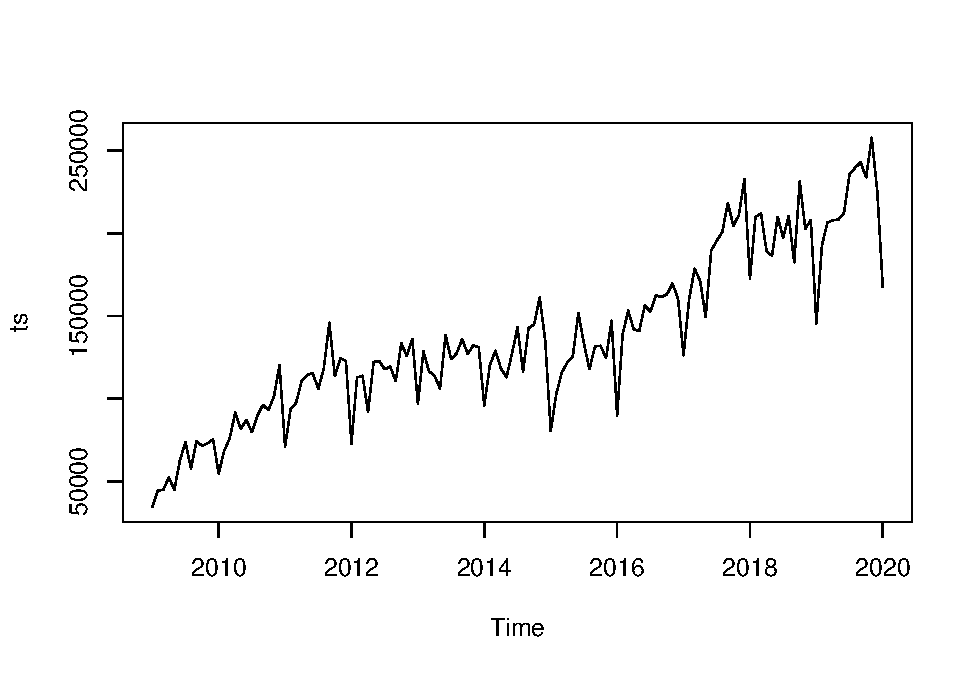
\includegraphics{tsf_export_files/figure-latex/unnamed-chunk-4-1.pdf}

In this case, it appears that an additive model is not appropriate for
describing this time series, since the size of the seasonal fluctuations
and random fluctuations seem to increase with the level of the time
series. Thus, we may need to transform the time series in order to get a
transformed time series that can be described using an additive model.
For example, we can transform the time series by calculating the natural
log of the original data:

\begin{Shaded}
\begin{Highlighting}[]
\NormalTok{log_ts <-}\StringTok{ }\KeywordTok{log}\NormalTok{(ts)}
\KeywordTok{plot.ts}\NormalTok{(log_ts)}
\end{Highlighting}
\end{Shaded}

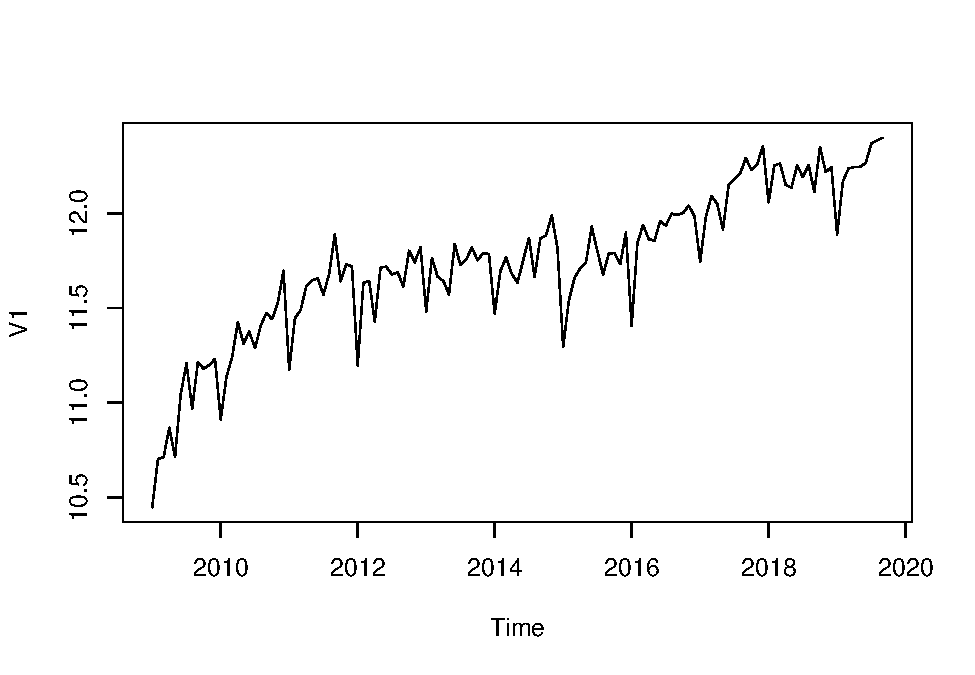
\includegraphics{tsf_export_files/figure-latex/unnamed-chunk-5-1.pdf}

\#\#Decomposing Time Series

Decomposing a time series means separating it into its constituent
components, which are usually a trend component and an irregular
component, and if it is a seasonal time series, a seasonal component.

\#\#\#Decomposing Seasonal Data A seasonal time series consists of a
trend component, a seasonal component and an irregular component.
Decomposing the time series means separating the time series into these
three components: that is, estimating these three components.

\begin{Shaded}
\begin{Highlighting}[]
\NormalTok{ts_components <-}\StringTok{ }\KeywordTok{decompose}\NormalTok{(ts)}
\end{Highlighting}
\end{Shaded}

we can print out the estimated values of the seasonal component

\begin{Shaded}
\begin{Highlighting}[]
\NormalTok{ts_components}\OperatorTok{$}\NormalTok{seasonal}
\end{Highlighting}
\end{Shaded}

\begin{verbatim}
##              Jan         Feb         Mar         Apr         May         Jun
## 2009 -35868.9712  -5110.0251    583.1592  -4870.7687  -7353.4162   7568.9602
## 2010 -35868.9712  -5110.0251    583.1592  -4870.7687  -7353.4162   7568.9602
## 2011 -35868.9712  -5110.0251    583.1592  -4870.7687  -7353.4162   7568.9602
## 2012 -35868.9712  -5110.0251    583.1592  -4870.7687  -7353.4162   7568.9602
## 2013 -35868.9712  -5110.0251    583.1592  -4870.7687  -7353.4162   7568.9602
## 2014 -35868.9712  -5110.0251    583.1592  -4870.7687  -7353.4162   7568.9602
## 2015 -35868.9712  -5110.0251    583.1592  -4870.7687  -7353.4162   7568.9602
## 2016 -35868.9712  -5110.0251    583.1592  -4870.7687  -7353.4162   7568.9602
## 2017 -35868.9712  -5110.0251    583.1592  -4870.7687  -7353.4162   7568.9602
## 2018 -35868.9712  -5110.0251    583.1592  -4870.7687  -7353.4162   7568.9602
## 2019 -35868.9712  -5110.0251    583.1592  -4870.7687  -7353.4162   7568.9602
## 2020 -35868.9712                                                            
##              Jul         Aug         Sep         Oct         Nov         Dec
## 2009   4706.4842   2153.8132   8726.0894   8919.6430   8748.6388  11796.3933
## 2010   4706.4842   2153.8132   8726.0894   8919.6430   8748.6388  11796.3933
## 2011   4706.4842   2153.8132   8726.0894   8919.6430   8748.6388  11796.3933
## 2012   4706.4842   2153.8132   8726.0894   8919.6430   8748.6388  11796.3933
## 2013   4706.4842   2153.8132   8726.0894   8919.6430   8748.6388  11796.3933
## 2014   4706.4842   2153.8132   8726.0894   8919.6430   8748.6388  11796.3933
## 2015   4706.4842   2153.8132   8726.0894   8919.6430   8748.6388  11796.3933
## 2016   4706.4842   2153.8132   8726.0894   8919.6430   8748.6388  11796.3933
## 2017   4706.4842   2153.8132   8726.0894   8919.6430   8748.6388  11796.3933
## 2018   4706.4842   2153.8132   8726.0894   8919.6430   8748.6388  11796.3933
## 2019   4706.4842   2153.8132   8726.0894   8919.6430   8748.6388  11796.3933
## 2020
\end{verbatim}

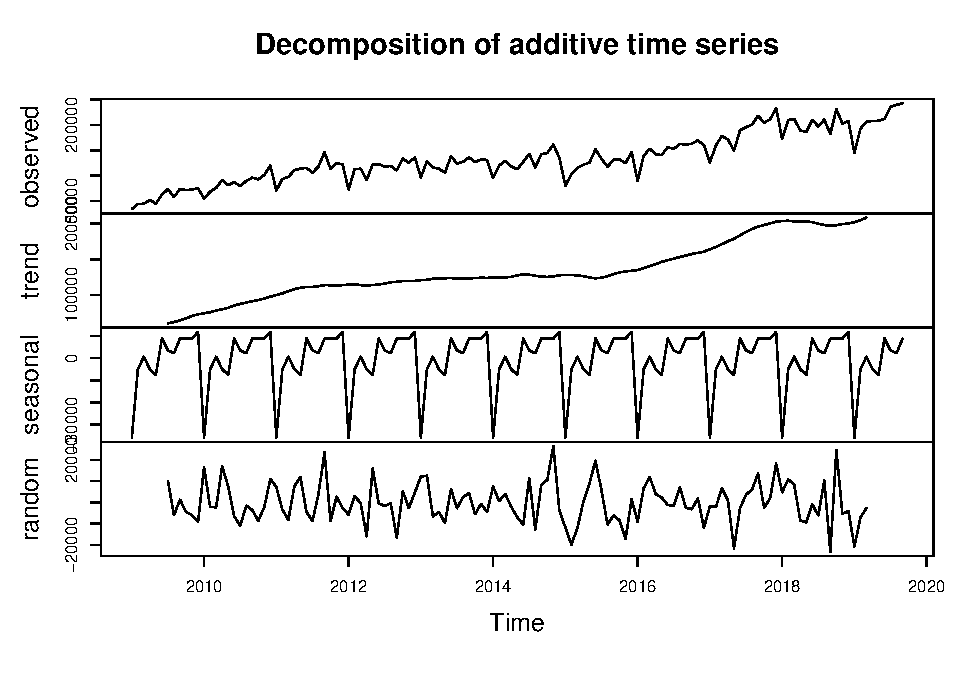
\includegraphics{tsf_export_files/figure-latex/unnamed-chunk-8-1.pdf}
The plot above shows the original time series (top), the estimated trend
component (second from top), the estimated seasonal component (third
from top), and the estimated irregular component (bottom)

\hypertarget{seasonally-adjusting}{%
\subsection{Seasonally Adjusting}\label{seasonally-adjusting}}

\begin{Shaded}
\begin{Highlighting}[]
\NormalTok{ts_seasonall <-}\StringTok{ }\NormalTok{ts }\OperatorTok{-}\StringTok{ }\NormalTok{ts_components}\OperatorTok{$}\NormalTok{seasonal}
\end{Highlighting}
\end{Shaded}

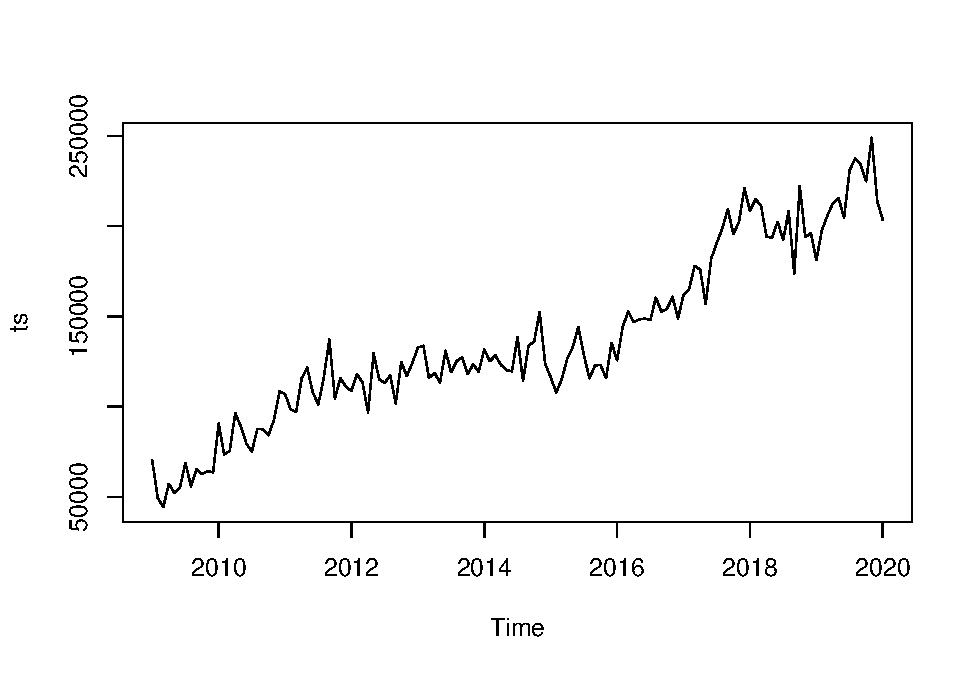
\includegraphics{tsf_export_files/figure-latex/unnamed-chunk-10-1.pdf}

\hypertarget{holt-winters-exponential-smoothing}{%
\subsection{Holt-Winters Exponential
Smoothing}\label{holt-winters-exponential-smoothing}}

\begin{Shaded}
\begin{Highlighting}[]
\NormalTok{ts_forcaste <-}\StringTok{ }\KeywordTok{HoltWinters}\NormalTok{(ts)}
\NormalTok{ts_forcaste}
\end{Highlighting}
\end{Shaded}

\begin{verbatim}
## Holt-Winters exponential smoothing with trend and additive seasonal component.
## 
## Call:
## HoltWinters(x = ts)
## 
## Smoothing parameters:
##  alpha: 0.3550801
##  beta : 0.01223594
##  gamma: 0.3718725
## 
## Coefficients:
##            [,1]
## a   227306.8042
## b     1573.4174
## s1   -7376.7400
## s2     343.7398
## s3   -7858.7490
## s4  -11901.5253
## s5    5357.7476
## s6    7156.3868
## s7    6538.0354
## s8    4815.7484
## s9    8180.6545
## s10   8364.9546
## s11   1449.0512
## s12 -50544.5232
\end{verbatim}

\begin{Shaded}
\begin{Highlighting}[]
\CommentTok{#}
\end{Highlighting}
\end{Shaded}

The value of alpha (0.35) is relatively low, indicating that the
estimate of the level at the current time point is based upon both
recent observations and some observations in the more distant past. The
value of beta is 0.01, indicating that the estimate of the slope b of
the trend component is updated but doesn't have much effect over the
time series, and instead is set equal to its initial value. This makes
good intuitive sense, as the level changes quite a bit over the time
series, but the slope b of the trend component remains roughly the same.
In contrast, the value of gamma (0.38) is high, indicating that the
estimate of the seasonal component at the current time point is not just
based upon very recent observations

\begin{Shaded}
\begin{Highlighting}[]
\NormalTok{ts_forcaste}\OperatorTok{$}\NormalTok{SSE}
\end{Highlighting}
\end{Shaded}

\begin{verbatim}
## [1] 23479926065
\end{verbatim}

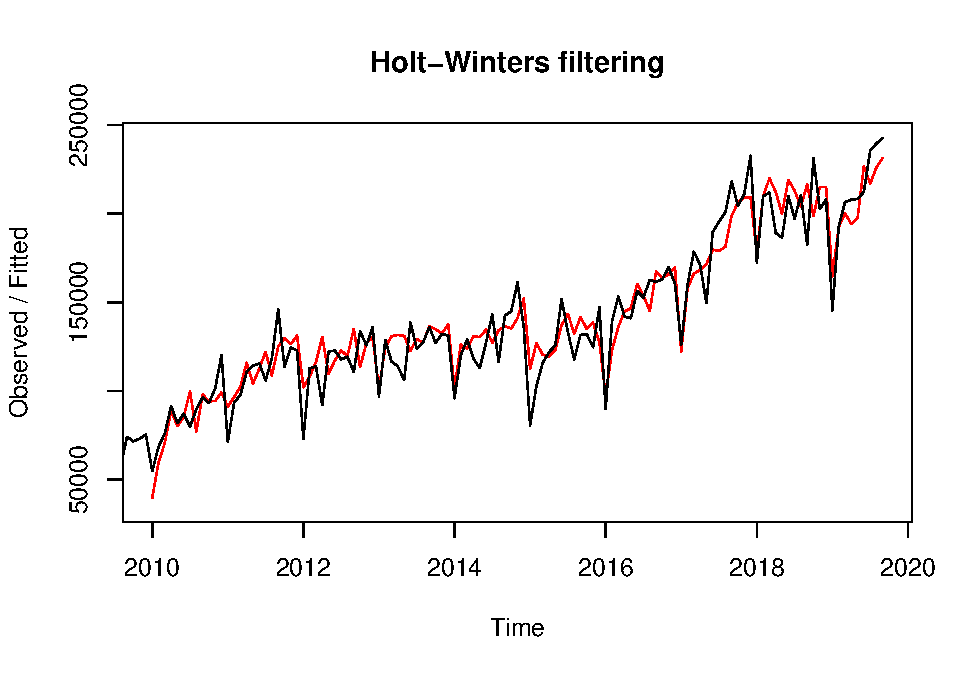
\includegraphics{tsf_export_files/figure-latex/unnamed-chunk-13-1.pdf}

\begin{Shaded}
\begin{Highlighting}[]
\NormalTok{ts_forcaste2 =}\StringTok{ }\NormalTok{forecast}\OperatorTok{:::}\KeywordTok{forecast.HoltWinters}\NormalTok{(ts_forcaste, }\DataTypeTok{h=} \DecValTok{11}\NormalTok{)}
\NormalTok{(}\KeywordTok{as.data.frame}\NormalTok{(ts_forcaste2))[}\DecValTok{1}\NormalTok{]}
\end{Highlighting}
\end{Shaded}

\begin{verbatim}
##          Point Forecast
## Feb 2020       221503.5
## Mar 2020       230797.4
## Apr 2020       224168.3
## May 2020       221698.9
## Jun 2020       240531.6
## Jul 2020       243903.7
## Aug 2020       244858.8
## Sep 2020       244709.9
## Oct 2020       249648.2
## Nov 2020       251405.9
## Dec 2020       246063.4
\end{verbatim}

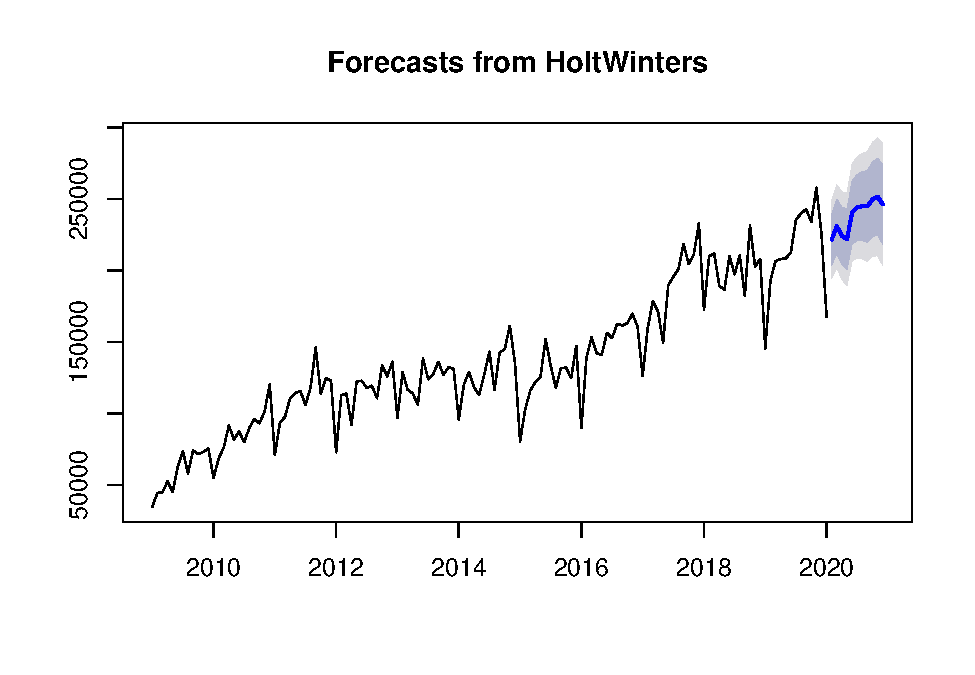
\includegraphics{tsf_export_files/figure-latex/unnamed-chunk-15-1.pdf}
\#\# Growth

\begin{Shaded}
\begin{Highlighting}[]
\NormalTok{year_}\DecValTok{2019}\NormalTok{ <-}\StringTok{ }\KeywordTok{window}\NormalTok{(ts, }\DecValTok{2019}\NormalTok{,}\KeywordTok{c}\NormalTok{(}\DecValTok{2019}\NormalTok{,}\DecValTok{12}\NormalTok{))}
\NormalTok{sum_year_}\DecValTok{2019}\NormalTok{ =}\StringTok{ }\KeywordTok{sum}\NormalTok{(}\KeywordTok{c}\NormalTok{(year_}\DecValTok{2019}\NormalTok{))}
\NormalTok{year_}\DecValTok{2020}\NormalTok{ =}\StringTok{ }\NormalTok{(}\KeywordTok{as.data.frame}\NormalTok{(ts_forcaste2))[}\DecValTok{1}\NormalTok{][}\KeywordTok{c}\NormalTok{(}\DecValTok{1}\OperatorTok{:}\DecValTok{11}\NormalTok{),]}
\NormalTok{sum_year_}\DecValTok{2020}\NormalTok{_HW <-}\KeywordTok{sum}\NormalTok{(}\KeywordTok{c}\NormalTok{(year_}\DecValTok{2020}\NormalTok{),}\KeywordTok{window}\NormalTok{(ts, }\DecValTok{2020}\NormalTok{))}
\NormalTok{growth_HW <-}\StringTok{ }\KeywordTok{growth}\NormalTok{(sum_year_}\DecValTok{2020}\NormalTok{_HW,sum_year_}\DecValTok{2019}\NormalTok{)}
\NormalTok{growth_HW}
\end{Highlighting}
\end{Shaded}

\begin{verbatim}
## [1] 0.06859268
\end{verbatim}

We can investigate whether the predictive model can be improved upon by
checking whether the in-sample forecast errors show non-zero
autocorrelations at lags 1-20, by making a correlogram and carrying out
the Ljung-Box test:

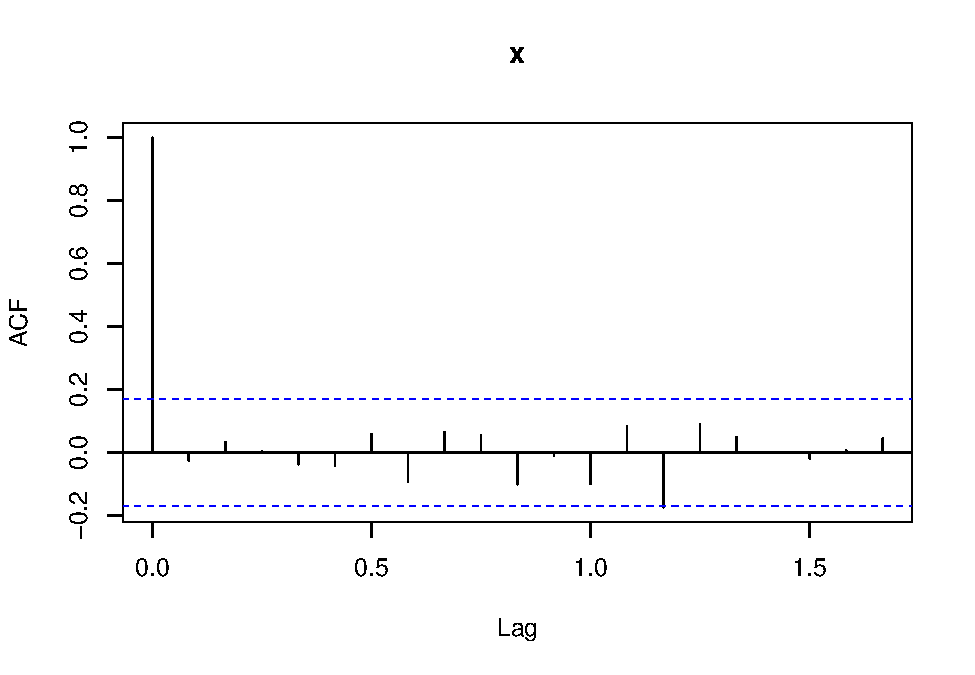
\includegraphics{tsf_export_files/figure-latex/unnamed-chunk-17-1.pdf}

\begin{verbatim}
## 
##  Box-Ljung test
## 
## data:  ts_forcaste2$residuals
## X-squared = 12.859, df = 20, p-value = 0.8834
\end{verbatim}

The correlogram shows that the autocorrelations for the in-sample
forecast errors do not exceed the significance bounds for lags 1-20.
Furthermore, the p-value for Ljung-Box test is 0.9, indicating that
there is no evidence of non-zero autocorrelations at lags 1-20.

We can check whether the forecast errors have constant variance over
time, and are normally distributed with mean zero, by making a time plot
of the forecast errors and a histogram (with overlaid normal curve):

\begin{Shaded}
\begin{Highlighting}[]
\KeywordTok{plot.ts}\NormalTok{(ts_forcaste2}\OperatorTok{$}\NormalTok{residuals)}
\end{Highlighting}
\end{Shaded}

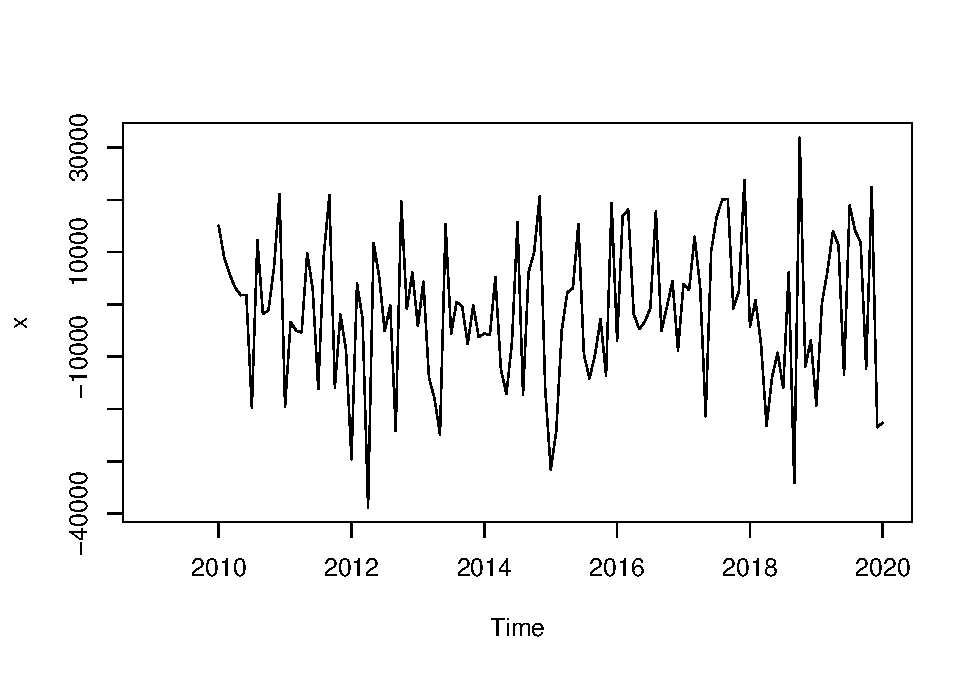
\includegraphics{tsf_export_files/figure-latex/unnamed-chunk-18-1.pdf}

\begin{Shaded}
\begin{Highlighting}[]
\CommentTok{# plotForecastErrors(ts_forcaste2$residuals)}
\end{Highlighting}
\end{Shaded}

From the time plot, it appears plausible that the forecast errors have
constant variance over time. From the histogram of forecast errors, it
seems plausible that the forecast errors are normally distributed with
mean zero.

Thus,there is little evidence of autocorrelation at lags 1-20 for the
forecast errors, and the forecast errors appear to be normally
distributed with mean zero and constant variance over time. This
suggests that Holt-Winters exponential smoothing provides an adequate
predictive model of the log of total productivity, which probably cannot
be improved upon. Furthermore, the assumptions upon which the prediction
intervals were based are probably valid.

\begin{Shaded}
\begin{Highlighting}[]
\KeywordTok{plot.ts}\NormalTok{(ts)}
\end{Highlighting}
\end{Shaded}

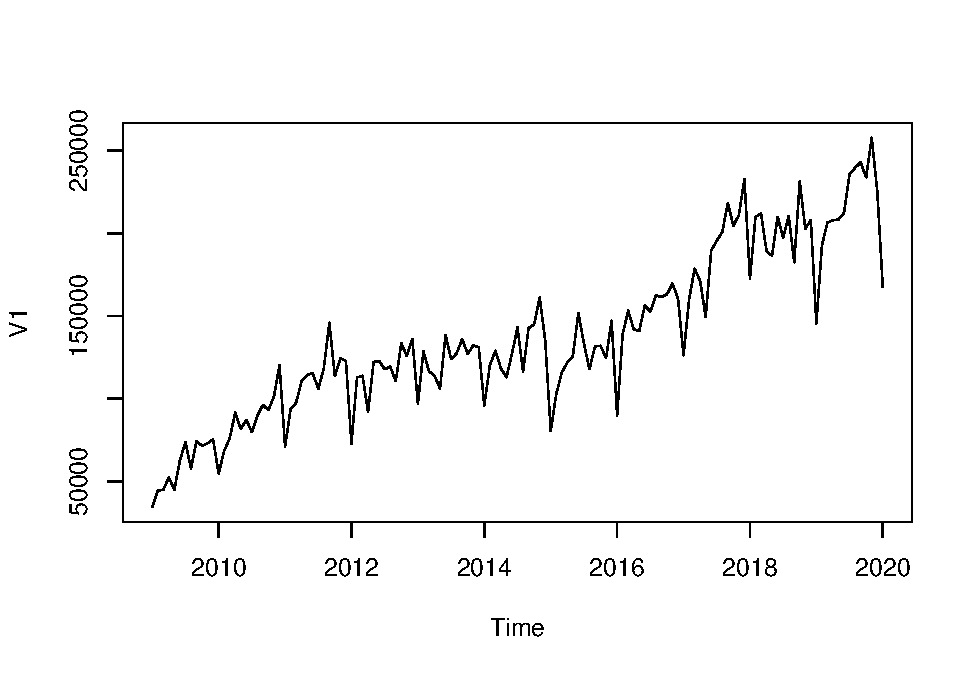
\includegraphics{tsf_export_files/figure-latex/unnamed-chunk-20-1.pdf}

\begin{Shaded}
\begin{Highlighting}[]
\NormalTok{ts_diff1 <-}\StringTok{  }\KeywordTok{diff}\NormalTok{(ts, }\DataTypeTok{differences =} \DecValTok{1}\NormalTok{)}

\KeywordTok{plot.ts}\NormalTok{(ts_diff1)}
\end{Highlighting}
\end{Shaded}

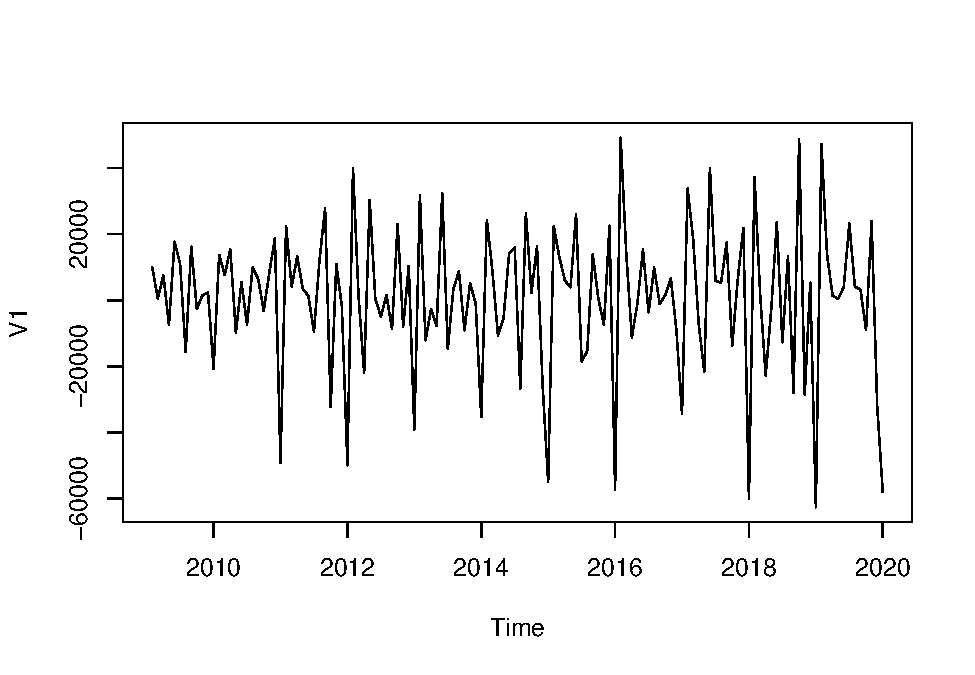
\includegraphics{tsf_export_files/figure-latex/unnamed-chunk-20-2.pdf}
The time series of differences (above) does appear to be stationary in
mean and variance, as the level of the series stays roughly constant
over time, and the variance of the series appears roughly constant over
time

\begin{Shaded}
\begin{Highlighting}[]
\KeywordTok{acf}\NormalTok{(ts_diff1, }\DataTypeTok{lag.max=}\DecValTok{20}\NormalTok{)             }\CommentTok{# plot a correlogram}
\end{Highlighting}
\end{Shaded}

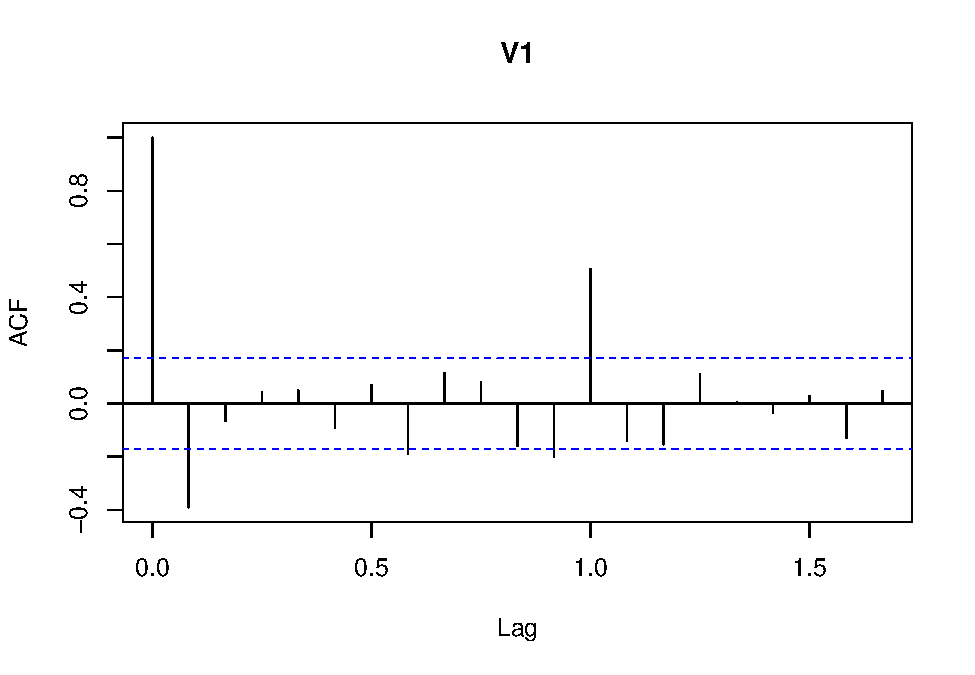
\includegraphics{tsf_export_files/figure-latex/unnamed-chunk-21-1.pdf}
We see from the correlogram that the autocorrelation exceeds the
significance bound 3 times but all the others do not exceed

\begin{Shaded}
\begin{Highlighting}[]
\KeywordTok{acf}\NormalTok{(ts_diff1, }\DataTypeTok{lag.max=}\DecValTok{20}\NormalTok{, }\DataTypeTok{plot=}\OtherTok{FALSE}\NormalTok{) }\CommentTok{# get the autocorrelation values}
\end{Highlighting}
\end{Shaded}

\begin{verbatim}
## 
## Autocorrelations of series 'ts_diff1', by lag
## 
## 0.0000 0.0833 0.1667 0.2500 0.3333 0.4167 0.5000 0.5833 0.6667 0.7500 0.8333 
##  1.000 -0.390 -0.066  0.041  0.049 -0.091  0.068 -0.188  0.113  0.079 -0.159 
## 0.9167 1.0000 1.0833 1.1667 1.2500 1.3333 1.4167 1.5000 1.5833 1.6667 
## -0.199  0.505 -0.141 -0.154  0.109  0.003 -0.035  0.029 -0.129  0.046
\end{verbatim}

\begin{Shaded}
\begin{Highlighting}[]
\KeywordTok{pacf}\NormalTok{(ts_diff1, }\DataTypeTok{lag.max=}\DecValTok{20}\NormalTok{)             }\CommentTok{# plot a partial correlogram}
\end{Highlighting}
\end{Shaded}

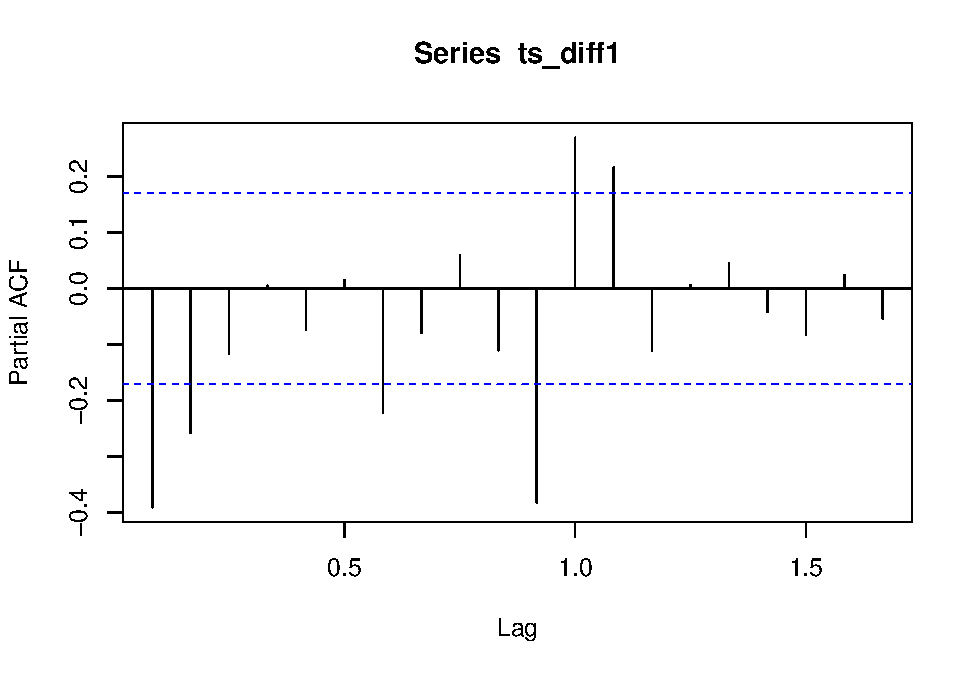
\includegraphics{tsf_export_files/figure-latex/unnamed-chunk-23-1.pdf}

\begin{Shaded}
\begin{Highlighting}[]
\KeywordTok{pacf}\NormalTok{(ts_diff1, }\DataTypeTok{lag.max=}\DecValTok{20}\NormalTok{, }\DataTypeTok{plot=}\OtherTok{FALSE}\NormalTok{) }\CommentTok{# get the partial autocorrelation values}
\end{Highlighting}
\end{Shaded}

\begin{verbatim}
## 
## Partial autocorrelations of series 'ts_diff1', by lag
## 
## 0.0833 0.1667 0.2500 0.3333 0.4167 0.5000 0.5833 0.6667 0.7500 0.8333 0.9167 
## -0.390 -0.258 -0.116  0.005 -0.074  0.015 -0.222 -0.078  0.060 -0.110 -0.382 
## 1.0000 1.0833 1.1667 1.2500 1.3333 1.4167 1.5000 1.5833 1.6667 
##  0.270  0.216 -0.110  0.006  0.046 -0.042 -0.082  0.025 -0.054
\end{verbatim}

\hypertarget{arima-010}{%
\section{Arima, 0,1,0}\label{arima-010}}

\begin{Shaded}
\begin{Highlighting}[]
\NormalTok{ts_arima =}\StringTok{ }\KeywordTok{Arima}\NormalTok{(ts, }\DataTypeTok{order=}\KeywordTok{c}\NormalTok{(}\DecValTok{1}\NormalTok{,}\DecValTok{1}\NormalTok{,}\DecValTok{1}\NormalTok{),}\DataTypeTok{seasonal =} \KeywordTok{list}\NormalTok{(}\DataTypeTok{order =} \KeywordTok{c}\NormalTok{(}\DecValTok{1}\NormalTok{,}\DecValTok{1}\NormalTok{,}\DecValTok{1}\NormalTok{)))}
\NormalTok{ts_arima}
\end{Highlighting}
\end{Shaded}

\begin{verbatim}
## Series: ts 
## ARIMA(1,1,1)(1,1,1)[12] 
## 
## Coefficients:
##          ar1      ma1     sar1     sma1
##       0.0199  -0.6250  -0.1612  -0.7249
## s.e.  0.1551   0.1227   0.1207   0.1065
## 
## sigma^2 estimated as 178190944:  log likelihood=-1314.33
## AIC=2638.66   AICc=2639.19   BIC=2652.6
\end{verbatim}

\begin{Shaded}
\begin{Highlighting}[]
\NormalTok{ts_arima_forecast =}\StringTok{ }\KeywordTok{forecast}\NormalTok{(ts_arima,}\DataTypeTok{h =} \DecValTok{11}\NormalTok{)}
\NormalTok{ts_arima_forecast}
\end{Highlighting}
\end{Shaded}

\begin{verbatim}
##          Point Forecast    Lo 80    Hi 80    Lo 95    Hi 95
## Feb 2020       217750.2 200638.1 234862.4 191579.4 243921.0
## Mar 2020       226899.4 208501.1 245297.6 198761.7 255037.0
## Apr 2020       218520.2 198990.3 238050.1 188651.8 248388.7
## May 2020       214394.1 193795.9 234992.3 182891.8 245896.4
## Jun 2020       235437.7 213824.0 257051.5 202382.3 268493.1
## Jul 2020       233673.6 211089.9 256257.3 199134.8 268212.4
## Aug 2020       236843.1 213329.5 260356.8 200882.1 272804.1
## Sep 2020       237924.8 213516.6 262332.9 200595.7 275253.9
## Oct 2020       246072.2 220801.1 271343.3 207423.4 284721.0
## Nov 2020       244826.2 218720.7 270931.6 204901.3 284751.0
## Dec 2020       246327.3 219413.3 273241.3 205165.9 287488.8
\end{verbatim}

\begin{Shaded}
\begin{Highlighting}[]
\NormalTok{forecast}\OperatorTok{:::}\KeywordTok{plot.forecast}\NormalTok{(ts_arima_forecast)}
\end{Highlighting}
\end{Shaded}

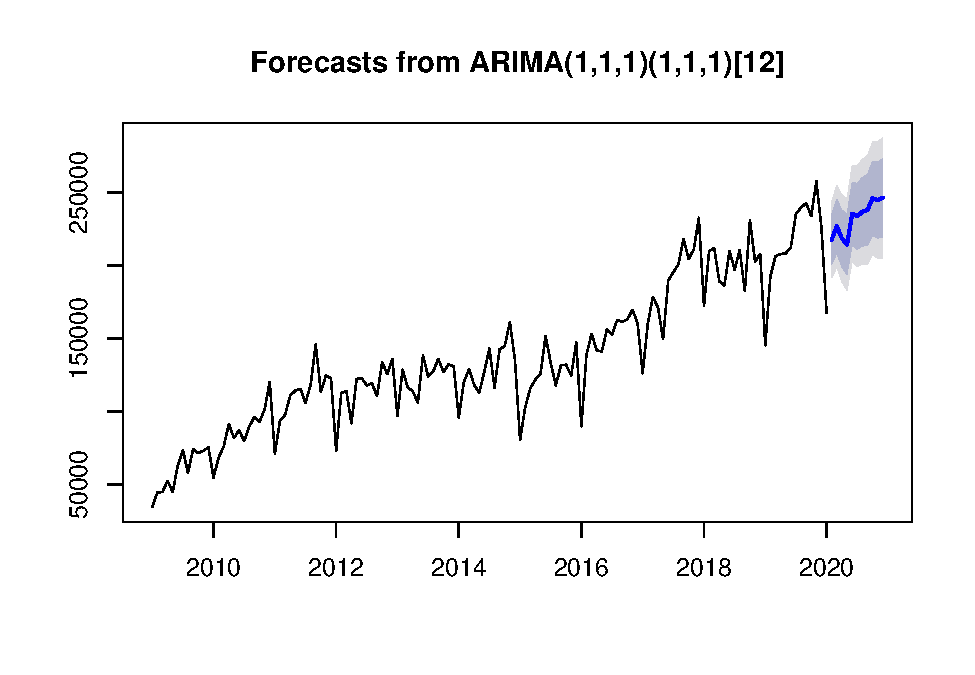
\includegraphics{tsf_export_files/figure-latex/unnamed-chunk-25-1.pdf}

\hypertarget{growth}{%
\subsection{Growth}\label{growth}}

\begin{Shaded}
\begin{Highlighting}[]
\CommentTok{# this_year_predict_ARIMA <- (as.data.frame(ts_arima_forecast))[1]}

\CommentTok{# growth_ARIMA <- growth(sum(c(this_year,as.numeric(this_year_predict_ARIMA$`Point Forecast`))), sum(last_year))}
\CommentTok{# growth_ARIMA}


\CommentTok{# year_2019_predict_ARIMA <- (as.data.frame(ts_arima_forecast))[1][c(1),]}
\CommentTok{# sum_year_2019 = sum(c(year_2019))}
\NormalTok{year_}\DecValTok{2020}\NormalTok{ =}\StringTok{ }\NormalTok{(}\KeywordTok{as.data.frame}\NormalTok{(ts_arima_forecast))[}\DecValTok{1}\NormalTok{][}\KeywordTok{c}\NormalTok{(}\DecValTok{1}\OperatorTok{:}\DecValTok{11}\NormalTok{),]}
\NormalTok{sum_year_}\DecValTok{2020}\NormalTok{_ARIMA =}\StringTok{ }\KeywordTok{sum}\NormalTok{(}\KeywordTok{c}\NormalTok{(year_}\DecValTok{2020}\NormalTok{,}\KeywordTok{window}\NormalTok{(ts,}\DecValTok{2020}\NormalTok{)))}
\NormalTok{growth_ARIMA <-}\StringTok{ }\KeywordTok{growth}\NormalTok{(sum_year_}\DecValTok{2020}\NormalTok{_ARIMA,sum_year_}\DecValTok{2019}\NormalTok{)}
\NormalTok{growth_ARIMA }
\end{Highlighting}
\end{Shaded}

\begin{verbatim}
## [1] 0.04534847
\end{verbatim}

As in the case of exponential smoothing models, it is a good idea to
investigate whether the forecast errors of an ARIMA model are normally
distributed with mean zero and constant variance, and whether the are
correlations between successive forecast errors.

For example, we can make a correlogram of the forecast errors for our
ARIMA(0,1,1) model, and perform the Ljung-Box test for lags 1-20, by
typing:

\begin{Shaded}
\begin{Highlighting}[]
\KeywordTok{acf}\NormalTok{(ts_arima_forecast}\OperatorTok{$}\NormalTok{residuals, }\DataTypeTok{lag.max=}\DecValTok{20}\NormalTok{)}
\end{Highlighting}
\end{Shaded}

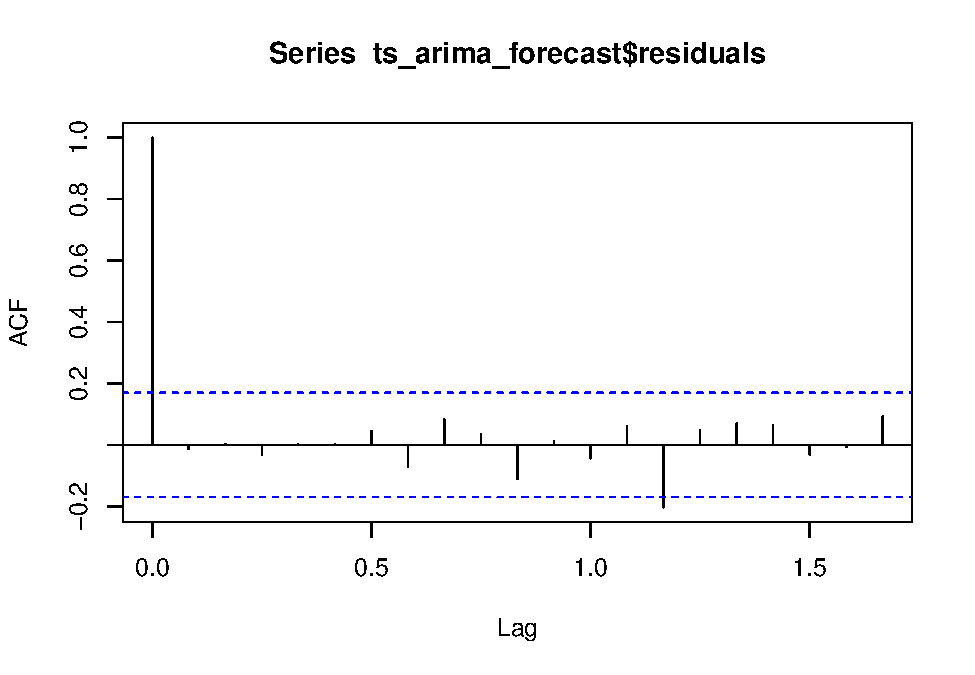
\includegraphics{tsf_export_files/figure-latex/unnamed-chunk-27-1.pdf}

\begin{Shaded}
\begin{Highlighting}[]
\KeywordTok{Box.test}\NormalTok{(ts_arima_forecast}\OperatorTok{$}\NormalTok{residuals, }\DataTypeTok{lag=}\DecValTok{20}\NormalTok{, }\DataTypeTok{type=}\StringTok{"Ljung-Box"}\NormalTok{)}
\end{Highlighting}
\end{Shaded}

\begin{verbatim}
## 
##  Box-Ljung test
## 
## data:  ts_arima_forecast$residuals
## X-squared = 14.401, df = 20, p-value = 0.8096
\end{verbatim}

\hypertarget{p-value-too-high-to-reject}{%
\section{p value too high to reject}\label{p-value-too-high-to-reject}}

\begin{Shaded}
\begin{Highlighting}[]
\KeywordTok{plot.ts}\NormalTok{(ts_arima_forecast}\OperatorTok{$}\NormalTok{residuals)            }\CommentTok{# make time plot of forecast errors}
\end{Highlighting}
\end{Shaded}

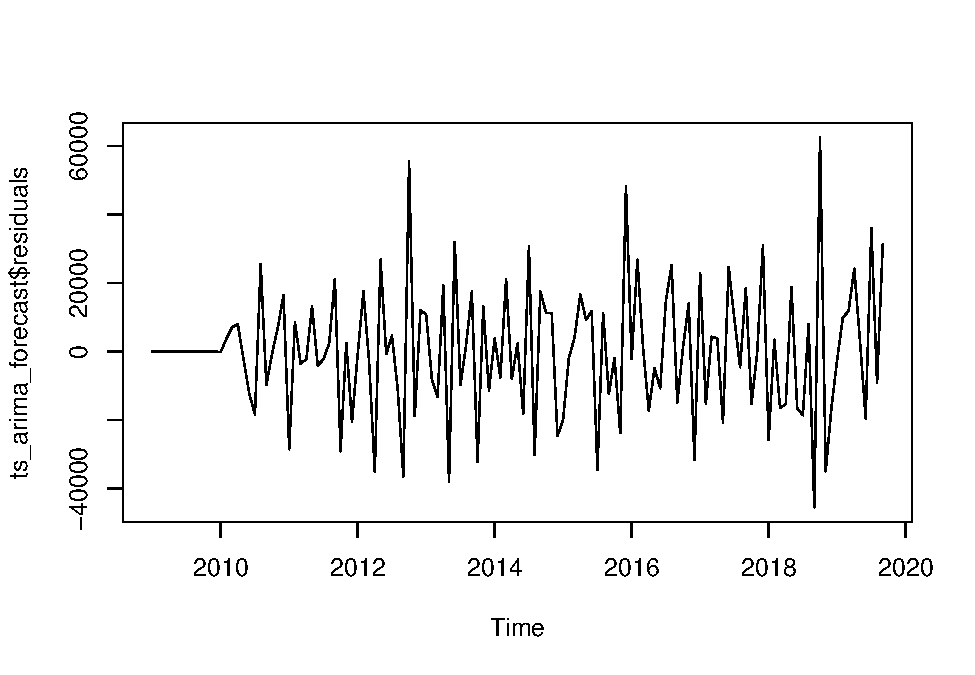
\includegraphics{tsf_export_files/figure-latex/unnamed-chunk-28-1.pdf}

\begin{Shaded}
\begin{Highlighting}[]
\KeywordTok{plotForecastErrors}\NormalTok{(ts_arima_forecast}\OperatorTok{$}\NormalTok{residuals)}
\end{Highlighting}
\end{Shaded}

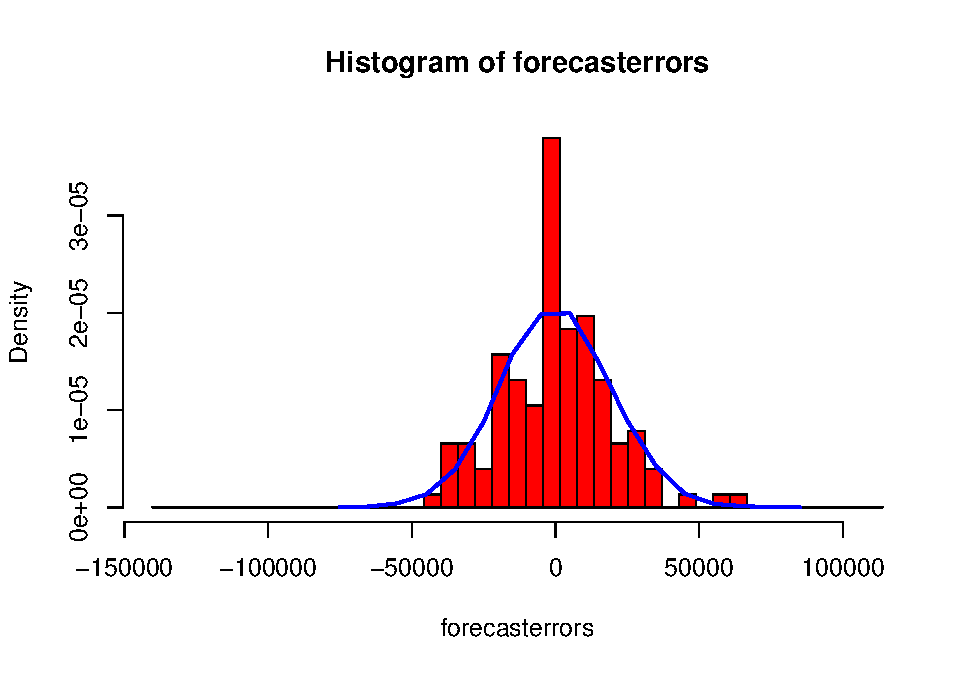
\includegraphics{tsf_export_files/figure-latex/unnamed-chunk-28-2.pdf}

\hypertarget{a-model-chosen-automatically}{%
\section{A model chosen
automatically}\label{a-model-chosen-automatically}}

\begin{Shaded}
\begin{Highlighting}[]
\NormalTok{fit3 <-}\StringTok{ }\KeywordTok{auto.arima}\NormalTok{(ts)}
\NormalTok{fit3}
\end{Highlighting}
\end{Shaded}

\begin{verbatim}
## Series: ts 
## ARIMA(1,0,1)(0,1,1)[12] with drift 
## 
## Coefficients:
##          ar1      ma1     sma1      drift
##       0.9348  -0.5736  -0.8165  1208.7731
## s.e.  0.0435   0.0962   0.0938   177.2516
## 
## sigma^2 estimated as 172154591:  log likelihood=-1323.51
## AIC=2657.03   AICc=2657.55   BIC=2671.01
\end{verbatim}

\begin{Shaded}
\begin{Highlighting}[]
\NormalTok{fit_forecast =}\StringTok{ }\KeywordTok{forecast}\NormalTok{(fit3,}\DataTypeTok{h=}\DecValTok{11}\NormalTok{)}
\KeywordTok{plot}\NormalTok{(fit_forecast)}
\end{Highlighting}
\end{Shaded}

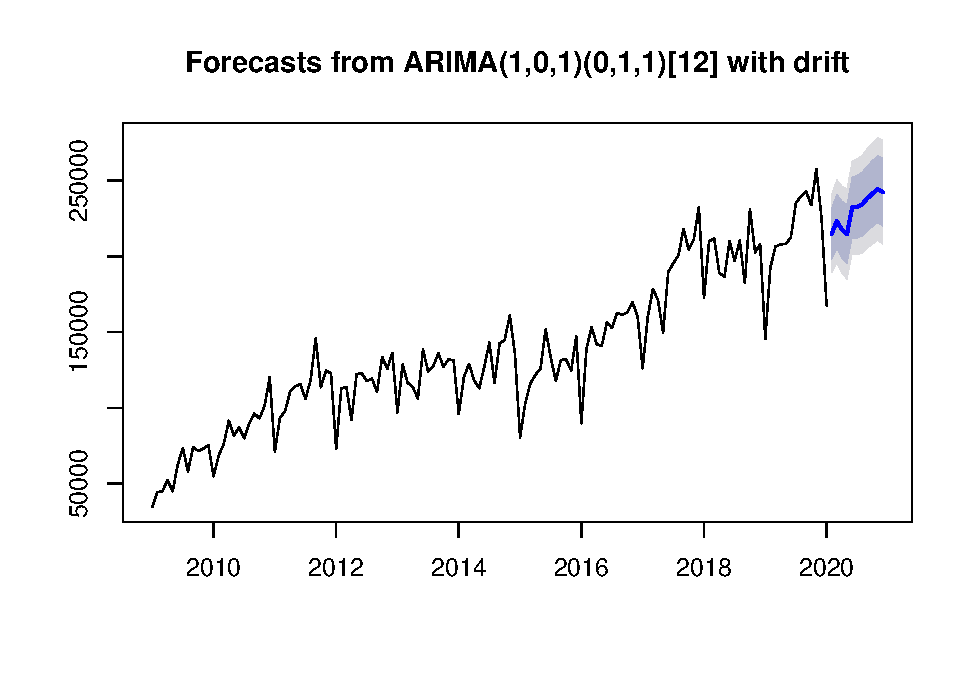
\includegraphics{tsf_export_files/figure-latex/unnamed-chunk-29-1.pdf}

\begin{Shaded}
\begin{Highlighting}[]
\CommentTok{# str(fit)}
\end{Highlighting}
\end{Shaded}

\hypertarget{growth-1}{%
\subsection{Growth}\label{growth-1}}

\begin{Shaded}
\begin{Highlighting}[]
\CommentTok{# year_2019 <- window(ts, 2019)}
\CommentTok{# year_2019_predict_HW <- (as.data.frame(ts_forcaste2))[1][c(1),]}
\CommentTok{# sum_year_2019 = sum(c(year_2019))}
\CommentTok{# year_2020 = (as.data.frame(ts_forcaste2))[1][c(2:13),]}


\CommentTok{# year_2019_predict_auto.arima <- (as.data.frame(fit_forecast))[1][c(1),]}
\CommentTok{# year_2019_predict_auto.arima_95_low <- (as.data.frame(fit_forecast))[4][c(1),]}
\CommentTok{# year_2019_predict_auto.arima_95_high <- (as.data.frame(fit_forecast))[5][c(1),]}

\CommentTok{# sum_year_2019 = sum(c(year_2019))}
\CommentTok{# sum_year_2019_low = sum(c(year_2019,year_2019_predict_auto.arima_95_low))}
\CommentTok{# sum_year_2019_high = sum(c(year_2019,year_2019_predict_auto.arima_95_high))}


\NormalTok{year_}\DecValTok{2020}\NormalTok{_predict_auto.arima <-}\StringTok{ }\NormalTok{(}\KeywordTok{as.data.frame}\NormalTok{(fit_forecast))[}\DecValTok{1}\NormalTok{][}\KeywordTok{c}\NormalTok{(}\DecValTok{1}\OperatorTok{:}\DecValTok{11}\NormalTok{),]}
\CommentTok{# year_2020_predict_auto.arima_95_low <- (as.data.frame(fit_forecast))[4][c(2:13),]}
\CommentTok{# year_2020_predict_auto.arima_95_high <- (as.data.frame(fit_forecast))[5][c(2:13),]}

\NormalTok{sum_year_}\DecValTok{2020}\NormalTok{_auto.ARIMA =}\StringTok{ }\KeywordTok{sum}\NormalTok{(}\KeywordTok{c}\NormalTok{(year_}\DecValTok{2020}\NormalTok{_predict_auto.arima,}\KeywordTok{window}\NormalTok{(ts,}\DecValTok{2020}\NormalTok{)))}

\NormalTok{growth_auto.arima <-}\StringTok{ }\KeywordTok{growth}\NormalTok{(sum_year_}\DecValTok{2020}\NormalTok{_auto.ARIMA,sum_year_}\DecValTok{2019}\NormalTok{)}
\CommentTok{# growth_auto.arima_95_low <- growth(sum(year_2020_predict_auto.arima_95_low),sum_year_2019_low)}
\CommentTok{# growth_auto.arima_95_high <- growth(sum(year_2020_predict_auto.arima_95_high),sum_year_2019_high)}

\NormalTok{growth_auto.arima}
\end{Highlighting}
\end{Shaded}

\begin{verbatim}
## [1] 0.03690604
\end{verbatim}

\begin{Shaded}
\begin{Highlighting}[]
\CommentTok{# growth_auto.arima_95_low}
\CommentTok{# growth_auto.arima_95_high}
\end{Highlighting}
\end{Shaded}

\end{document}
